%!TEX root=ClassNotes.tex

\section{Applications of Integrals}

\subsection{Improper Integrals}
Improper integrals compute areas of unbounded regions. These integrals are a source of several false paradoxes. As we'll see below, counter-intuitive as it may seem, unbounded regions {\it can} have finite areas.\\

We'll study two types of improper integrals: depending on whether the corresponding region is unbounded along the $x$-axis or along the $y$-axis.
The idea is to {\it view an unbounded region as a limit of bounded regions}.

\begin{definition}
  {\bf Improper integrals} (of the first kind) are integrals where one (or both) of the bounds is $\pm \infty$.\footnote{Note that $\infty$ is not a number here either, but represents a limit.}
  Let $f$ be a continuous function.
  Define,
	\begin{align*}
		\int \limits_a^{\infty} f(t) \: dt
		 & =
		\lim \limits_{x \rightarrow \infty}\int \limits_a^{x} f(t) \: dt \\
		\int \limits_{-\infty}^a f(t) \: dt
		 & =
		\lim \limits_{x \rightarrow -\infty}\int \limits_{x}^{a} f(t) \: dt \\
		\int \limits_{-\infty}^{\infty} f(t) \: dt
		 & =
		\lim \limits_{x \rightarrow \infty}\int \limits_0^{x} f(t) \: dt
    +
    \lim \limits_{x \rightarrow -\infty}\int \limits_{x}^{0} f(t) \: dt
	\end{align*}
  where $a$ is a real number.
\end{definition}

\begin{exercise}
	For the following problems, draw the region whose area the integral is computing (you can use a calculator for graphing) and compute the integral.
	\begin{multicols}{2}
		\begin{enumerate}
			\item $\int \limits_1^{\infty} \dfrac{1}{t} \: dt$
			\item $\int \limits_1^{\infty} \dfrac{1}{t^2} \: dt$
			\item $\int \limits_0^{\infty} \sin t \: dt$
			\item $\int \limits_0^{\infty} 2t e^{-t^2} \: dt$
			\item $\int \limits_{1}^{\infty} \dfrac{9}{(1 - 3t)^4} \: dt$
			\item $\int \limits_{-\infty}^{\infty} \dfrac{6 t^3}{(t^4 + 1)^2} \: dt$
		\end{enumerate}
	\end{multicols}
\end{exercise}

\begin{exercise}
  \begin{enumerate}
    \item The choice of the number 0 in the definition of $\int_{-\infty}^{\infty}$ is not important. We can replace 0 with any real number and the answer would not change.
    Compute
    \begin{align*}
      \lim \limits_{x \rightarrow \infty}\int \limits_1^{x} \dfrac{6 t^3}{(t^4 + 1)^2} \: dt
      +
      \lim \limits_{x \rightarrow -\infty}\int \limits_{x}^1 \dfrac{6 t^3}{(t^4 + 1)^2} \: dt
    \end{align*}
    and compare it with Problem 6 of the previous exercise. Why does the answer not change?

    \item On the other hand, consider the following change.
    Compute
    \begin{enumerate}
      \item $\lim \limits_{x \rightarrow \infty}\int \limits_{-x}^{x} \sin t \: dt$, and
      \item $\lim \limits_{x \rightarrow \infty}\int \limits_0^{x} \sin t \: dt
      +
      \lim \limits_{x \rightarrow -\infty}\int \limits_{x}^{0} \sin t \: dt$
    \end{enumerate}
    Why are the two answers different?
  \end{enumerate}
  Thus, when limits are involved, our intuition does not always provide us with the correct answer.
\end{exercise}

\begin{definition}
  {\bf Improper integrals} (of the second kind) are integrals where the function being integrated has a discontinuity in the interval of integration.
  Let $[a,b]$ be an interval and let $c \in [a, b]$ be a point such that $f(x)$ is discontinuous at $c$ but continuous on the rest of interval. Define,
	\begin{align*}
    \mbox{if } a < c < b, &&
    \int \limits_a^b f(t) \: dt
		 & =
		\lim \limits_{x \rightarrow c^{-}}\int \limits_a^{x} f(t) \: dt
    +
    \lim \limits_{x \rightarrow c^{+}}\int \limits_{x}^{b} f(t) \: dt \\
    \mbox{if } c = a, &&
    \int \limits_c^b f(t) \: dt
		 & =
    \lim \limits_{x \rightarrow c^{+}}\int \limits_{x}^{b} f(t) \: dt \\
    \mbox{if } c = b, &&
    \int \limits_a^c f(t) \: dt
		 & =
		\lim \limits_{x \rightarrow c^{-}}\int \limits_a^{x} f(t) \: dt
	\end{align*}
\end{definition}


\begin{exercise}
	For the following problems, draw the region whose area the integral is computing (you can use a calculator for graphing if you like) and compute the integral.
	\begin{multicols}{2}
		\begin{enumerate}
			\item $\int \limits_0^{3} \dfrac{1}{\sqrt{3 - t}} \: dt$
			\item $\int \limits_{2}^{3} \dfrac{4t}{\sqrt[3]{t^2 - 4}} \: dt$
			\end{enumerate}
	\end{multicols}
\end{exercise}

It is possible to compute integrals of more general unbounded regions using the same ideas.

\subsection{Arc Length}
Recall that the integral $\int_a^b f(t) \: dt$ is defined as the limit of the Riemann sum
\begin{align*}
  \sum_{i = 0}^{n-1} m_i (x_{i+1} - x_{i})
\end{align*}
where $x_i$'s form a partition of the interval $[a,b]$ and $m_i$ is the min (inf) of the $f(x)$ values in the interval $[x_i, x_{i+1}]$. One way to {\it represent} this sum is as the sum of several quantities of the form
\begin{align*}
  y \: \Delta x
\end{align*}
where $\Delta x$ stands for the length of the interval $x_{i+1} - x_i$ which can be thought of as {\bf the change in $x$}, and $y$ stands for {\bf the minimum value of $f(x)$} for $x \in[x_i, x_{i+1}]$. So that
\begin{align}
  \label{eq:sum_limit}
  \lim \limits_{\Delta x \rightarrow 0} \left(\sum y \: \Delta x \right) = \int y \: dx
\end{align}
The reason for doing this, is that this allows us to interpret several {\it naturally occurring} quantities as integrals (which is why the Riemann sum formulation of integral is much more useful than the area formulation). One such example is an {\bf arc length}.\\


{\bf Arc length} is just a fancy name for the length of a curve. For example, the arc length of a circle of radius $r$ is $2 \pi r$. We are interested in computing the arc length of the graph of a function $y=f(x)$.
\begin{figure}[H]
  \centering
  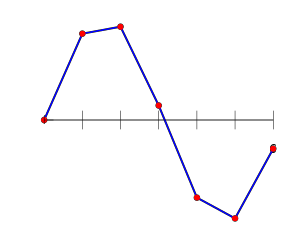
\includegraphics[width=0.5\textwidth]{ArcLength.png}
  \caption*{Approximating the graph $y=f(x)$ by line segments}
\end{figure}
We do this by partitioning the interval $[a,b]$ and approximating the graph $ y = f(x)$ over each partition by a straight line. The length of each small straight line segment equals
\begin{align*}
  \sqrt{\Delta x^2 + \Delta y^2}
\end{align*}
and hence the arc length equals
\begin{align*}
  \lim \limits_{\Delta x \rightarrow 0}  \left(\sum \sqrt{\Delta x^2 + \Delta y^2}\right)
\end{align*}
This looks very close to \eqref{eq:sum_limit}. Next we need to separate a $\Delta x$ term.
\begin{align*}
  \lim \limits_{\Delta x \rightarrow 0} \left(\sum \sqrt{1 + \left(\dfrac{\Delta y}{\Delta x}\right)^2} \Delta x \right)
\end{align*}
This looks exactly like \eqref{eq:sum_limit} with $y$ replaced with $\sqrt{1 + \left(\frac{\Delta y}{\Delta x}\right)^2}$. Finally we notice that
\begin{align*}
  \lim \limits_{\Delta x \rightarrow 0} \dfrac{\Delta y}{\Delta x} = \dfrac{dy}{dx}
\end{align*}
which gives us the formula for the arc length.
\begin{theorem}
  \label{thm:arclength}
  Let $f$ be a differentiable function on the interval $[a,b]$. The arc length of the graph $y = f(x)$ over the interval $[a,b]$ is given by the integral
  \begin{align*}
    \int \limits_a^b \sqrt{1 + \left(\dfrac{dy}{dx} \right)^2}  \: dx
  \end{align*}
\end{theorem}
While the above derivation is not a {\it proof}, it can be converted into a proof using $\sup$'s and $\inf$'s, using the same method we used to prove the Fundamental Theorem of Calculus.

\begin{exercise}
  Using the arc length formula in Theorem \ref{thm:arclength} compute the following:
  \begin{enumerate}
    \item Circumference of a circle of radius r.
    \item Arc length of the parabola $y = x^2$ from 0 to 1.
    \item Arc length of line segment $y = m x$ from $a$ to $b$, where $m$, $a$, $b$ are real numbers. Explain the result geometrically.
  \end{enumerate}
\end{exercise}

\begin{exercise}
  Here we encounter the first example of a {\it naturally occurring} unsolvable integral.
  Find the expression for the arc length of the sine curve $y = \sin x$ from 0 to $a$.
  This integral, called an {\bf elliptic integral}, cannot be algebraically computed.\footnote{Even though elliptic integrals cannot be simplified algebraically, they have deep connections to number theory.
  The impossibility of algebraically evaluating elliptic integrals presents the first obstacle towards a complete understanding of prime numbers!\\
  See: \url{https://en.wikipedia.org/wiki/Elliptic_function}}
\end{exercise}

\begin{exercise}{\bf (Optional)}
  In this problem, you'll need to use the fact that the (curved) surface area of a cylinder is $2 \pi r h$ and the volume is $\pi r^2 h$, where $r$ is the radius and $h$ is the height of the cylinder.
  \begin{figure}[H]
    \centering
    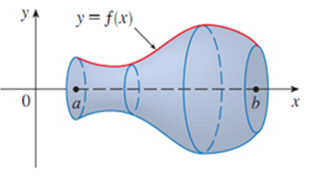
\includegraphics[width=0.5\textwidth]{SurfaceOfRevolution.png}
  \end{figure}
  \end{exercise}
  \begin{enumerate}
    \item Derive the formula for the area of the surface obtained by revolving the curve $y = f(x)$ over the interval $[a,b]$ about the $x$-axis.
   Such a surface is called a {\bf surface of revolution}.
    \item Derive the formula for the volume of the solid obtained by revolving the region under the curve $y = f(x)$ over the interval $[a,b]$ about the $x$-axis.
    Such a solid is called a {\bf solid of revolution}.
  \end{enumerate}
We can do both of these constructions by revolving the curve about the $y$-axis instead of the $x$-axis. In this case, we simply switch $x$ and $y$ and use the function $x=f^{-1}(y)$ instead of $y = f(x)$.\\


\subsection{Differential Equations}
It would be remiss to not mention differential equations while studying applications of calculus.
Calculus was invented by Newton to find solutions to his laws of motion, which are a set of differential equations.

A {\bf differential equation} is any equation involving derivatives $\frac{dy}{dx}$, $\frac{d^2y}{dx^2}$ etc.
Solving a differential equation means finding a function $y = f(x)$ that satisfies the equation.

We've already encountered one very simple differential equation.
The Fundamental Theorem of Calculus is essentially a statement about the solution of a differential equation.
We can rephrase it as saying:\\ {\it The solution to the differential equation
\begin{align*}
  \dfrac{dy}{dx} = g(x)
\end{align*}
is given by
\begin{align*}
  y = \int g(x) \: dx.
\end{align*}
}

In this section, we'll see some examples of differential equations without going into any details.
It is not possible to {\it solve} this differential equation in the same way that we solve algebraic equations. Instead, we {\it guess} a solution and verify it.

\begin{exercise}
  A {\bf separable} differential equation is of the form
  \begin{align*}
    \dfrac{dy}{dx} = f(x) \cdot g(y)
  \end{align*}
  for some functions $f$ and $g$. The solution of this differential equation is given by
  \begin{align*}
    \int \dfrac{1}{g(y)} \: dy  = \int f(x) \: dx
  \end{align*}
  It is called separable because the variables $x$ and $y$ can be ``separated'' i.e. all the terms involving $y$ are on the left hand side and all the terms involving $x$ are on the right hand side. A non-example is $\frac{dy}{dx} = x + y$.

  Find solutions for the following separable differential equations and verify that your solution satisfies the differential equation.
  \begin{multicols}{2}
    \begin{enumerate}
      \item $\dfrac{dy}{dx} = 2y$
      \item $\dfrac{dy}{dx} = xy$
      \item $\dfrac{dy}{dx} = \dfrac{3x^2}{\cos y}$
      \item $\dfrac{dy}{dx} = - \dfrac{y}{x}$
      \item $\dfrac{dy}{dx} = - \dfrac{x}{y}$
      \item $\dfrac{dy}{dx} = e^{-y}(2x - 4) $
    \end{enumerate}
  \end{multicols}
\end{exercise}

\newpage
\begin{exercise}
  The following differential equation is called a {\bf damped harmonic oscillator},
  \begin{align*}
    m \dfrac{d^2y}{dx^2} + c \dfrac{dy}{dx} + k y = 0
  \end{align*}
  where $m$, $k$, and $c$ are constants.
  This differential equation is used to model simple oscillatory systems.
  \begin{enumerate}
    \item Find a number(s) $r$ such that $y=e^{rx}$ solves the differential equation
    \begin{align*}
       \dfrac{d^2y}{dx^2} - 4 y = 0
    \end{align*}
    \item Find a number(s) $r$ such that $y=e^{rx}$ solves the differential equation
    \begin{align*}
       \dfrac{d^2y}{dx^2} + 4 y = 0
    \end{align*}
    \item Find a number(s) $r$ such that $y=e^{rx}$ solves the differential equation
    \begin{align*}
       \dfrac{d^2y}{dx^2} - 2 \dfrac{dy}{dx} + y = 0
    \end{align*}
    For this $r$, verify that $y = x e^{rx}$ is also a solution.
    \item Notice that the three equations have very different kinds of solutions.
    How would you describe the difference between the three equations?
  \end{enumerate}
\end{exercise}

Differential equations in general are very very difficult to solve. Finding solutions to differential equations has been a guiding question for much of modern mathematics. It is still not known whether a solution exists to the differential equation that describes fluid motion.\footnote{See \url{https://en.wikipedia.org/wiki/Navier-Stokes_equations}.} Nevertheless a lot of techniques now exist for solving a variety of differential equations either exactly or numerically.
Differential equations is one of the most active areas of mathematical research today.
